\documentclass[a4paper,12pt]{article}
\usepackage{standalone}
\usepackage{amsmath} % Package for advanced math typesetting
\input{../../sty/setup.sty} % Assuming these files exist and are correctly referenced
\graphicspath{ {../../pictures/IDMA/IDMA_4a}} % Assuming a pictures folder has been made and is correctly referenced

% \renewcommand{\thesection}{5.\arabic{section}} % Substitue 5. for any number

% Changes sections from 1.1 to 1.a
\renewcommand{\thesubsection}{\thesection.\alph{subsection}}

\begin{document}
% \includepdf[pages=-]{../../pictures/forside}

\title{Københavns Universitet\\
Introduktion til diskret matematik og algoritmer - Problem set 3}
\author{Victor Vangkilde Jørgensen - kft410\\ 
kft410@alumni.ku.dk}
\makeatletter
\let\getauthor\@author
\let\gettitle\@title
\makeatother
\maketitle
\thispagestyle{empty}
\n\n
 % Assuming this file contains the cover page setup

\pagebreak
\pagestyle{empty}
\tableofcontents
\pagebreak
\pagestyle{fancy}
\fancyhf{}
\setlength{\headheight}{15.2pt}
\renewcommand{\footrulewidth}{0.4pt}
\fancyhead[R]{\nouppercase \lastrightmark}
\fancyfoot[L]{\gettitle}
\fancyfoot[R]{\thepage}
 % Assuming this file contains the header setup
\maketitle % This command will actually insert the title into the document



\section[Question 1]{}
\begin{figure}[H]
    \centering
    \includegraphics[width=0.9\textwidth]{1.png}
    \caption{Directed graph $G$ for which to compute strongly connected components in Problem 1a.}
\end{figure}

\subsection[]{}
Vi opskriver vores directed graph som en adjacency list representation i lexicographic order:
\[
\begin{aligned}
&a \rightarrow (b, d, e)\\
&b \rightarrow (a, c, d)\\
&c \rightarrow (a, e, f)\\
&d \rightarrow (e, f)\\
&e \rightarrow (d, f, h)\\
&f \rightarrow (g)\\
&g \rightarrow (h)\\
&h \rightarrow (f)\\
\end{aligned}
\]

\begin{figure}[h]
    \centering
    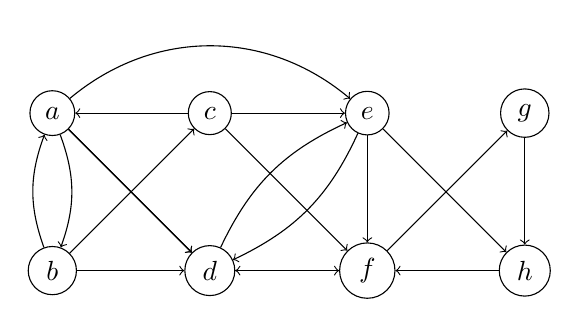
\begin{tikzpicture}
        \node[circle, draw] (a) at (0,2) {$a$};
        \node[circle, draw] (b) at (0,0) {$b$};
        \node[circle, draw] (c) at (2,2) {$c$};
        \node[circle, draw] (d) at (2,0) {$d$};
        \node[circle, draw] (e) at (4,2) {$e$};
        \node[circle, draw] (f) at (4,0) {$f$};
        \node[circle, draw] (g) at (6,2) {$g$};
        \node[circle, draw] (h) at (6,0) {$h$};
        \draw[->] (b) -- (d);
        \draw[->] (c) -- (a);
        \draw[->] (c) -- (e);
        \draw[->] (d) -- (f);
        \draw[->] (e) -- (f);
        \draw[->] (e) -- (h);
        \draw[->] (f) -- (d);
        \draw[->] (g) -- (h);
        \draw[->] (h) -- (f);
        \draw[->] (f) -- (g);
        \draw[->] (a) -- (d);
        \draw[->] (a) -- (d);
        \draw[->] (c) -- (f);
        \draw[->] (b) -- (c);
        \draw[->] (a) to[bend left=20] (b);
        \draw[->] (b) to[bend left=20] (a);
        \draw[->] (a) to[bend left=40] (e);
        \draw[->] (d) to[bend left=20] (e);
        \draw[->] (e) to[bend left=20] (d);
    \end{tikzpicture}
    \caption*{}
    \end{figure}
\subsection[]{}



\begin{figure}[H]
    \centering
    \includegraphics[width=1\textwidth]{2.png}
    \caption{}
\end{figure}
\section[Question 2]{}
\subsection[]{}



\subsection[]{}



\subsection[]{}



\subsection[]{}



\begin{figure}[H]
    \centering
    \includegraphics[width=0.8\textwidth]{3.png}
    \caption{Directed graph Dijkstra's algorithm in Problem 3a.}
\end{figure}
\section[Question 3]{}
\subsection[]{}

Jeg opskriver vores weighted directed graph som adjacency list representation $(vertex, weight)$:
\[
\begin{aligned}
&(a,0) \rightarrow ((b,1), (d,5), (e,6), (g,9))\\
&(b,0) \rightarrow ((c,1), (e,2), (f,9))\\
&(c,0) \rightarrow ((e,4), (f,7))\\
&(d,0) \rightarrow ((e,6), (g,5), (h,2))\\
&(e,0) \rightarrow ((f,5), (h,4))\\
&(f,0) \rightarrow (e,3)\\
&(g,0) \rightarrow ()\\
&(h,0) \rightarrow (f,1)\\
\end{aligned}
\]

Udregning af distancer for $a's$ naboer:
\[
[(b,1),(d,5),(e,6),(g,9)]
\]
Vi opdaterer nu de laveste værdier i grafen:
\[
[(A,0),(b,1),(c,\infty),(d,5),(e,6),(f,\infty),(g,9),(h,\infty)]
\]
$a$ er nu besøgt, så det har jeg markeret ved at skrive $A$ i stedet.\\
\[
\begin{tikzpicture}[heap]
    \node {$(A,0)$}
        child{node{$(b,1)$}
            child{node{$(e,6)$} child{node{$(h,\infty)$}}} 
            child{node{$(g,9)$}}}
        child{node{$(d,5)$}
            child{node{$(c,\infty)$}} 
            child{node{$(f,\infty)$}}}
    ;
\end{tikzpicture}
\]

Vi ser, at $b$ er den ubesøgte vertex med kortest afstand fra $a.$\\
Udregning af nye distancer for $b's$ naboer:
\[
[(c,1+1),(e,1+2),(f,1+9)] = [(c,2),(e,3),(f,10)]
\]
Vi opdaterer nu de laveste værdier i grafen:
\[
[(A,0),(B,1),(c,2),(e,3),(d,5),(g,9),(f,10),(h,\infty)]
\]
$b$ er nu besøgt, så det har jeg markeret ved at skrive $B$ i stedet.\\

Vi ser, at $c$ er den ubesøgte vertex med kortest afstand fra $a$.\\
Udregning af nye distancer for $c's$ naboer:
\[
[(e,2+4),(f,2+7)] = [(e,6),(f,9)]
\]
Vi opdaterer nu de laveste værdier i grafen:
\[
[(A,0),(B,1),(C,2),(e,3),(d,5),(f,9),(g,9),(h,\infty)]
\]
$c$ er nu besøgt, så det har jeg markeret ved at skrive $C$ i stedet.\\

Vi ser, at $e$ er den ubesøgte vertex med kortest afstand fra $a$.\\
Udregning af nye distancer for $e's$ naboer:
\[
[(f,3+5),(h,3+4)] = [(f,8),(h,7)]
\]
Vi opdaterer nu de laveste værdier i grafen:
\[
[(A,0),(B,1),(C,2),(E,3),(d,5),(h,7),(f,8),(g,9)]
\]
$e$ er nu besøgt, så det har jeg markeret ved at skrive $E$ i stedet.\\

Vi ser, at $d$ er den ubesøgte vertex med kortest afstand fra $a$.\\
Udregning af nye distancer for $d's$ naboer:
\[
[(g,5+5),(h,5+5),(e,5+6)] = [(g,10),(h,10),(e,11)]
\]
Vi opdaterer nu de laveste værdier i grafen, men ser, at der ikke nogen kortere afstande:
\[
[(A,0),(B,1),(C,2),(E,3),(D,5),(h,7),(f,8),(g,9)]
\]
$d$ er nu besøgt, så det har jeg markeret ved at skrive $D$ i stedet.\\

Vi ser, at $h$ er den ubesøgte vertex med kortest afstand fra $a$.\\
Udregning af nye distancer for $h's$ naboer:
\[
[(f,7+1)] = [(f,8)]
\]
Vi opdaterer nu de laveste værdier i grafen, men ser, at der ikke nogen kortere afstande:
\[
[(A,0),(B,1),(C,2),(E,3),(D,5),(H,7),(f,8),(g,9)]
\]
$h$ er nu besøgt, så det har jeg markeret ved at skrive $H$ i stedet.\\

Vi ser, at $f$ er den ubesøgte vertex med kortest afstand fra $a$.\\
Udregning af nye distancer for $f's$ naboer:
\[
[(e,8+3)] = [(e,11)]
\]
Vi opdaterer nu de laveste værdier i grafen, men ser, at der ikke nogen kortere afstande:
\[
[(A,0),(B,1),(C,2),(E,3),(D,5),(H,7),(F,8),(g,9)]
\]
$f$ er nu besøgt, så det har jeg markeret ved at skrive $F$ i stedet.\\

Vi ser, at $g$ er den sidste ubesøgte vertex, og at $g$ ikke har nogen naboer.\\
\[
[(A,0),(B,1),(C,2),(E,3),(D,5),(H,7),(F,8),(G,9)]
\]
Vi markerer $g$ som besøgt med $G$.

\subsection[]{}



\subsection[]{}



\subsection[]{}



\end{document}